\documentclass[11pt,a4paper,landscape]{article}

\usepackage[a4paper,margin=0.55in]{geometry}
\usepackage[T1]{fontenc}
\usepackage[utf8]{inputenc}
\usepackage{xcolor}
\usepackage{tikz}
\usetikzlibrary{positioning,arrows.meta}

\pagestyle{empty}
\setlength{\parindent}{0pt}

\tikzset{
  relation/.style={
    draw,
    rounded corners=4pt,
    fill=blue!7,
    minimum height=2.5cm,
    text width=8cm,
    align=left,
    inner sep=8pt,
    font=\footnotesize
  },
  title/.style={
    font=\bfseries\footnotesize
  },
  link/.style={
    -{Latex[length=2.5mm]},
    thick,
    gray!75
  }
}

\begin{document}

\begin{center}
{\Large \textbf{Task 2 Schema Design}}\\[4pt]
{\small Relational schema derived from the improved ER diagram}
\end{center}

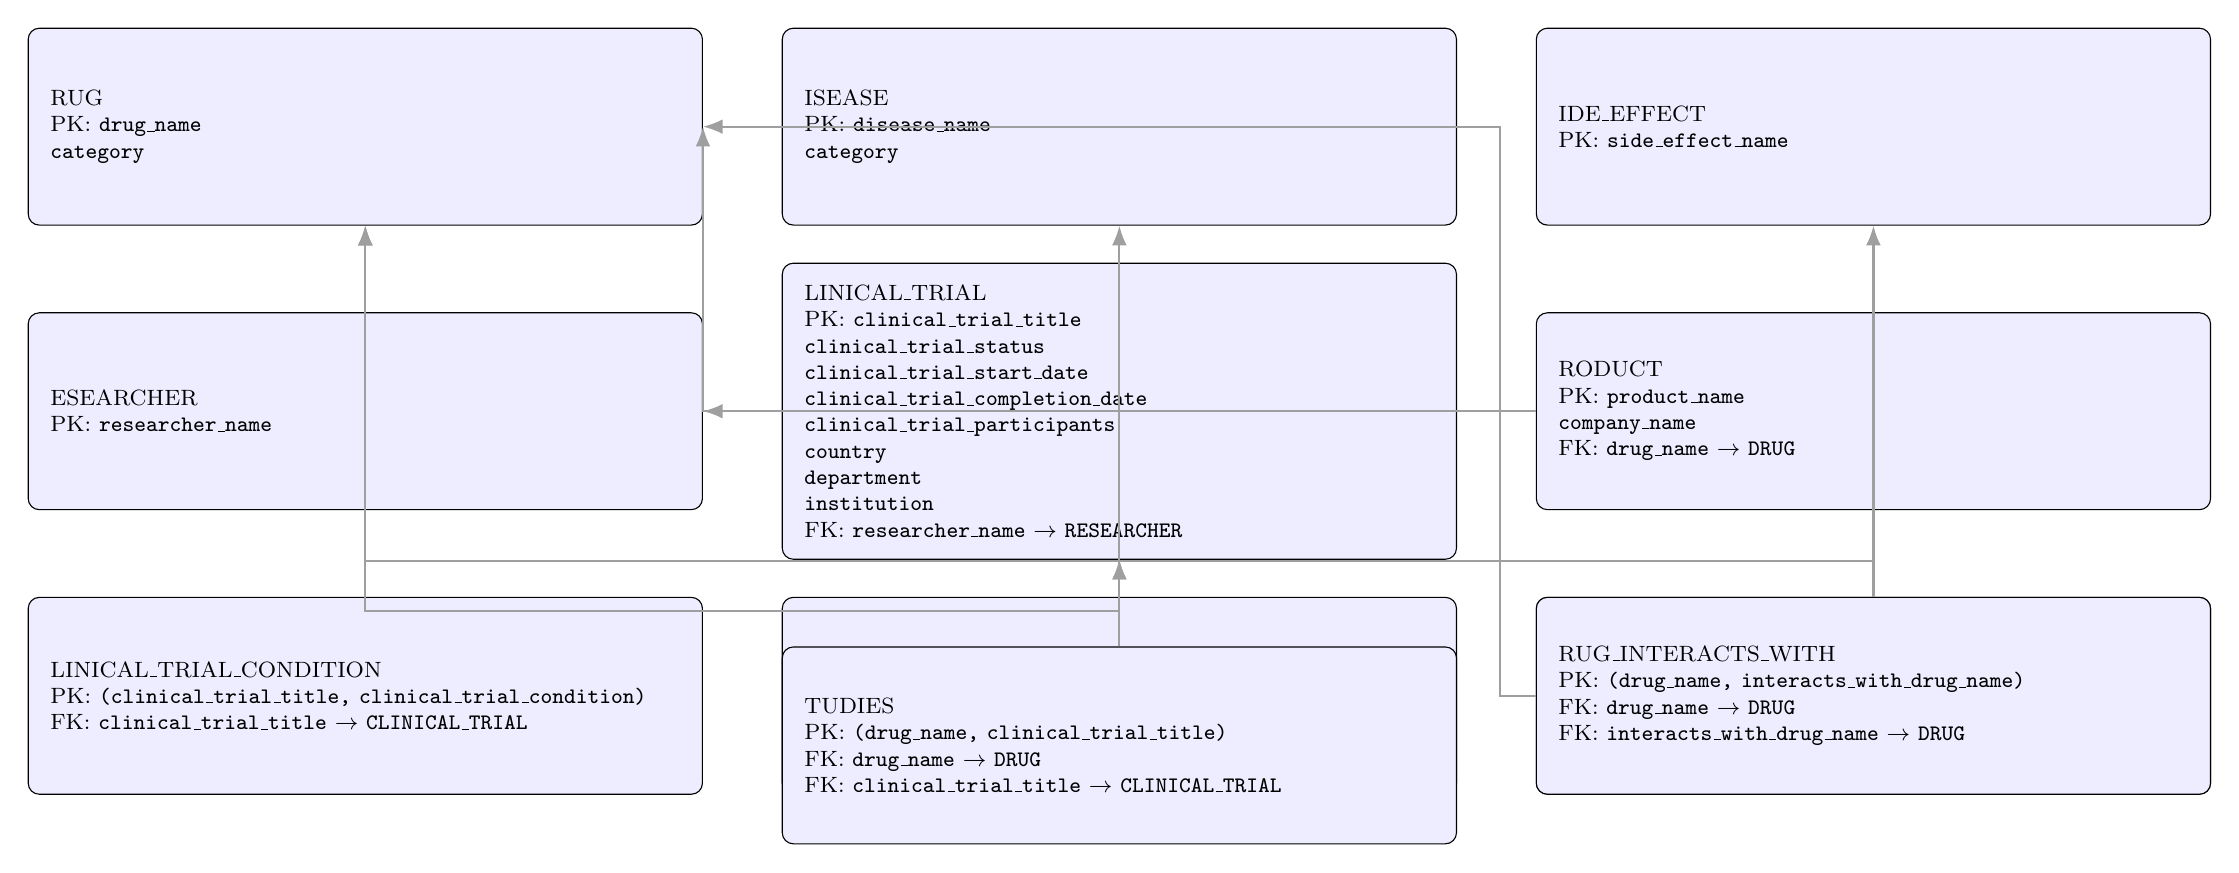
\begin{tikzpicture}[node distance=1.1cm and 1.0cm]

\node[relation] (drug) {
{\title DRUG}\\
PK: \texttt{drug\_name}\\
\texttt{category}
};

\node[relation, right=of drug] (disease) {
{\title DISEASE}\\
PK: \texttt{disease\_name}\\
\texttt{category}
};

\node[relation, right=of disease] (sideeffect) {
{\title SIDE\_EFFECT}\\
PK: \texttt{side\_effect\_name}
};

\node[relation, below=of drug] (researcher) {
{\title RESEARCHER}\\
PK: \texttt{researcher\_name}
};

\node[relation, right=of researcher] (trial) {
{\title CLINICAL\_TRIAL}\\
PK: \texttt{clinical\_trial\_title}\\
\texttt{clinical\_trial\_status}\\
\texttt{clinical\_trial\_start\_date}\\
\texttt{clinical\_trial\_completion\_date}\\
\texttt{clinical\_trial\_participants}\\
\texttt{country}\\
\texttt{department}\\
\texttt{institution}\\
FK: \texttt{researcher\_name} $\rightarrow$ \texttt{RESEARCHER}
};

\node[relation, right=of trial] (product) {
{\title PRODUCT}\\
PK: \texttt{product\_name}\\
\texttt{company\_name}\\
FK: \texttt{drug\_name} $\rightarrow$ \texttt{DRUG}
};

\node[relation, below=of researcher] (trialcondition) {
{\title CLINICAL\_TRIAL\_CONDITION}\\
PK: \texttt{(clinical\_trial\_title, clinical\_trial\_condition)}\\
FK: \texttt{clinical\_trial\_title} $\rightarrow$ \texttt{CLINICAL\_TRIAL}
};

\node[relation, right=of trialcondition] (treats) {
{\title TREATS}\\
PK: \texttt{(drug\_name, disease\_name)}\\
FK: \texttt{drug\_name} $\rightarrow$ \texttt{DRUG}\\
FK: \texttt{disease\_name} $\rightarrow$ \texttt{DISEASE}
};

\node[relation, right=of treats] (hasse) {
{\title HAS\_SIDE\_EFFECT}\\
PK: \texttt{(drug\_name, side\_effect\_name)}\\
FK: \texttt{drug\_name} $\rightarrow$ \texttt{DRUG}\\
FK: \texttt{side\_effect\_name} $\rightarrow$ \texttt{SIDE\_EFFECT}
};

\node[relation, below=of trial] (studies) {
{\title STUDIES}\\
PK: \texttt{(drug\_name, clinical\_trial\_title)}\\
FK: \texttt{drug\_name} $\rightarrow$ \texttt{DRUG}\\
FK: \texttt{clinical\_trial\_title} $\rightarrow$ \texttt{CLINICAL\_TRIAL}
};

\node[relation, below=of product] (interacts) {
{\title DRUG\_INTERACTS\_WITH}\\
PK: \texttt{(drug\_name, interacts\_with\_drug\_name)}\\
FK: \texttt{drug\_name} $\rightarrow$ \texttt{DRUG}\\
FK: \texttt{interacts\_with\_drug\_name} $\rightarrow$ \texttt{DRUG}
};

\draw[link] (trial.west) -- ++(-0.45,0) |- (researcher.east);
\draw[link] (trialcondition.north) -- ++(0,0.45) -| (trial.south);
\draw[link] (treats.north) -- ++(0,0.45) -| (drug.south);
\draw[link] (treats.north) -- ++(0,0.45) -| (disease.south);
\draw[link] (hasse.north) -- ++(0,0.45) -| (drug.south);
\draw[link] (hasse.north) -- ++(0,0.45) -| (sideeffect.south);
\draw[link] (studies.north) -- ++(0,0.45) -| (drug.south);
\draw[link] (studies.north) -- ++(0,0.45) -| (trial.south);
\draw[link] (product.west) -- ++(-0.45,0) -| (drug.east);
\draw[link] (interacts.west) -- ++(-0.45,0) |- (drug.east);

\end{tikzpicture}

\end{document}
